% 6×18 Strategy Taxonomy Diagram
% Generated for CCSE-CS paper
\begin{figure}[t]
\centering
\resizebox{\textwidth}{!}{
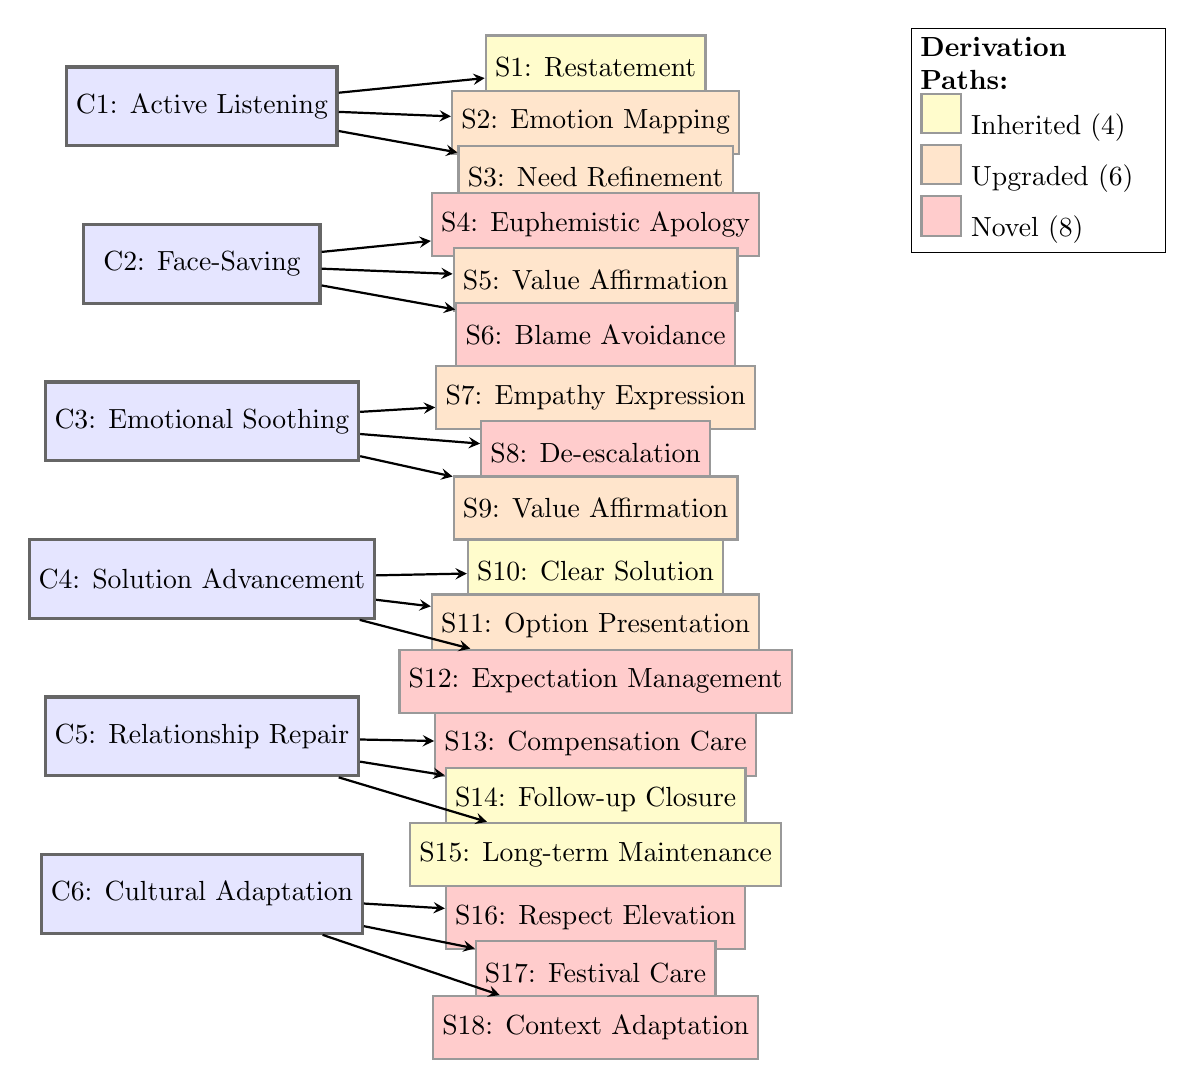
\begin{tikzpicture}[
    category/.style={rectangle, draw=black!60, fill=blue!10, very thick, minimum size=1cm, minimum width=3cm},
    strategy/.style={rectangle, draw=black!40, fill=green!10, thick, minimum size=0.8cm, minimum width=2.5cm},
    inherited/.style={strategy, fill=yellow!20},
    upgraded/.style={strategy, fill=orange!20},
    novel/.style={strategy, fill=red!20},
    arrow/.style={->, >=stealth, thick},
    label text/.style={font=\footnotesize\itshape}
]

% Categories (C1-C6)
\node[category] (C1) at (0, 8) {C1: Active Listening};
\node[category] (C2) at (0, 6) {C2: Face-Saving};
\node[category] (C3) at (0, 4) {C3: Emotional Soothing};
\node[category] (C4) at (0, 2) {C4: Solution Advancement};
\node[category] (C5) at (0, 0) {C5: Relationship Repair};
\node[category] (C6) at (0, -2) {C6: Cultural Adaptation};

% Strategies for C1
\node[inherited] (S1) at (5, 8.5) {S1: Restatement};
\node[upgraded] (S2) at (5, 7.8) {S2: Emotion Mapping};
\node[upgraded] (S3) at (5, 7.1) {S3: Need Refinement};

% Strategies for C2
\node[novel] (S4) at (5, 6.5) {S4: Euphemistic Apology};
\node[upgraded] (S5) at (5, 5.8) {S5: Value Affirmation};
\node[novel] (S6) at (5, 5.1) {S6: Blame Avoidance};

% Strategies for C3
\node[upgraded] (S7) at (5, 4.3) {S7: Empathy Expression};
\node[novel] (S8) at (5, 3.6) {S8: De-escalation};
\node[upgraded] (S9) at (5, 2.9) {S9: Value Affirmation};

% Strategies for C4
\node[inherited] (S10) at (5, 2.1) {S10: Clear Solution};
\node[upgraded] (S11) at (5, 1.4) {S11: Option Presentation};
\node[novel] (S12) at (5, 0.7) {S12: Expectation Management};

% Strategies for C5
\node[novel] (S13) at (5, -0.1) {S13: Compensation Care};
\node[inherited] (S14) at (5, -0.8) {S14: Follow-up Closure};
\node[inherited] (S15) at (5, -1.5) {S15: Long-term Maintenance};

% Strategies for C6
\node[novel] (S16) at (5, -2.3) {S16: Respect Elevation};
\node[novel] (S17) at (5, -3.0) {S17: Festival Care};
\node[novel] (S18) at (5, -3.7) {S18: Context Adaptation};

% Arrows from categories to strategies
\draw[arrow] (C1) -- (S1);
\draw[arrow] (C1) -- (S2);
\draw[arrow] (C1) -- (S3);
\draw[arrow] (C2) -- (S4);
\draw[arrow] (C2) -- (S5);
\draw[arrow] (C2) -- (S6);
\draw[arrow] (C3) -- (S7);
\draw[arrow] (C3) -- (S8);
\draw[arrow] (C3) -- (S9);
\draw[arrow] (C4) -- (S10);
\draw[arrow] (C4) -- (S11);
\draw[arrow] (C4) -- (S12);
\draw[arrow] (C5) -- (S13);
\draw[arrow] (C5) -- (S14);
\draw[arrow] (C5) -- (S15);
\draw[arrow] (C6) -- (S16);
\draw[arrow] (C6) -- (S17);
\draw[arrow] (C6) -- (S18);

% Legend
\node[draw, fill=white, anchor=north west] at (9, 9) {
    \begin{minipage}{3cm}
    \textbf{Derivation Paths:}\\
    \tikz\node[inherited, minimum size=0.5cm] {}; Inherited (4)\\
    \tikz\node[upgraded, minimum size=0.5cm] {}; Upgraded (6)\\
    \tikz\node[novel, minimum size=0.5cm] {}; Novel (8)
    \end{minipage}
};

\end{tikzpicture}
}
\caption{6×18 Strategy Taxonomy with three derivation paths: Inherited (directly from ESConv/CSC), Upgraded (refined from existing strategies), and Novel (culturally-derived for Chinese customer service).}
\label{fig:strategy_taxonomy}
\end{figure}
